\chapter{Approaches}
\label{ch:approaches}

The Thesis work follows the Deduction research approach as mentioned in chapter \ref{ch:background} where the theory is established based on own ideas in addition to literature review findings. In order to tackle the research questions, different disciplines of software engineering such as Complex datasets, Compiler reporting, Continuous integration, Refactoring tools, Issue tracker, Stack Overflow, Gamification, Usability Engineering etc. are looked into and studied what ideas can be adapted into our scenario along with own novel solution ideas.\\ \\

After the literature review in above-mentioned disciplines, here are a few important takeaways in the scope of this Thesis. In the area of 'Complex datasets', current research where Dix et. al. \cite{Dix} talks about more complex grouping and linking of datasets in the context of a user interface of Spreadsheets application. There could be two datasets with fields having similar meaning and fields which are completely different. So, the key takeaway is about design lessons of extensibility of columns for example, 'venues were geocoded to allow spatial graphs' could be related as an example dates in bug reports to some standard format for all tools used and shown on a unified interface. Next, Gaur et. al. \cite{Gaur} speaks about the linear search problem in indexing as it takes more time for large volumes of data. So, different parameters are introduced to decrease computation time. Example: a database with toys is searched linearly for a given query it takes more time than a modified query let's say a toy in red colour and type horse then the search is simplified by looking at two parameters i.e, colour and type. This sparks the idea of grouping bugs as per module, bug type which could ease user in finding a certain bug on an interface.  \\ \\

In the area of 'Compiler reporting', Horning et. al. \cite{horning} mentions the importance of error logging with statistics as to what the compilers are expected to tell the user. It also mentions, the importance of stating what kind of bugs are not found along with bugs found but in reality this questions the scalability. So, the key takeaway is it is ideal to show the number of certain bugs founds in an analysis. Next in the area of 'Refactoring tools', Dustinca \cite{dustinca} talks about how the Refactoring tools are to be built and in user context, it has to overcome the barrier of discoverability which means the difficulty of use. To assist the developer on this issue, they introduced a smart tag in the context of user editor and notifies which parts of the code can be refactored. This emphasizes the importance of 'on-board' phase which plays a key role in Gamification \cite{gamify} discipline. Hayashi et. al. \cite{Hayashi} illustrates the importance of task level commits in order to maintain edit history of refactorings. This gives an idea of which a user does a bug-fix level commit to addressing the traceability scenario. Mealy et. al. \cite{Mealy} mentions about the importance of usability for software refactoring tools and this could perhaps give some basic guidelines similar to knowing Usability Engineering \cite{usability} discipline. \\ \\

In the area of 'Issue tracker', Baysal et. al. \cite{Baysal} mentions reducing the information overload for a developer in using the issue tracker. It is found out in their there is a too much of information they receive which in fact confuses the developer in how to react, example: the developer receive a high number of bugs reported via email and this leads to a situation where the developer ignore the email. They found out some interesting solution ideas such as having a private dashboard for each developer as it becomes easy to react to issues correspond to them. Expressiveness is one other mentioned in their paper which says an example, severity or priority are vague terms to describe a bug. Perhaps, it is ideal to describe the priory as per team decision instead of personal choice.  This signifies in categorising the results as per categories in our unified interface. Next in 'Stack Overflow', in a research paper by Wang et. al. \cite{stack} it is found there are 10934198 questions on a 'User Interface' topic for example. It is quite challenging to go through such a high volume database but nevertheless, the Stack Overflow team has a friendly user interface as shown in the following figure \ref{fig:stackoverflow}. It uses some clean filter techniques like tags for each topic, priority and trending etc. A research by Treude et. al. \cite{Treude.2011} found out that most of the questions (72.30\%) in Stack Overflow have between 2 and 4 tags. This could perhaps ease in filtering/indexing issues. \\ \\

\begin{figure}[hbt!]
	\centering
	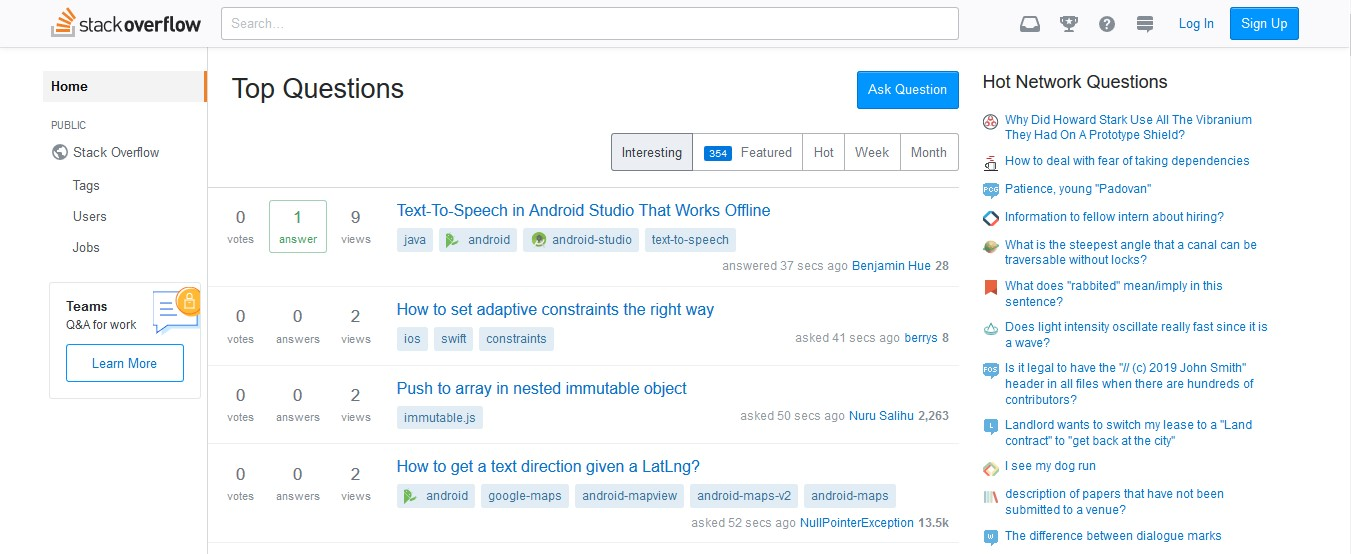
\includegraphics[width=\linewidth]{figures/stackoverflow}
	\caption{An user interface of Stack Overflow Website.}
	\label{fig:stackoverflow}
\end{figure}

Overall, by analysing the software engineering disciplines as mentioned above, a theory is established. The prototypes are created based on the established theory and user study mentioned in Evaluation chapter \ref{ch:evaluationplan} is performed which follows Qualitative and Quantitative approaches in assimilating the results. It follows a well established Iterative process of UX Design \cite{UX} cycle as seen in the figure \ref{fig:ux-design}. \\ \\

Our approach leads an iterative process where initially prototypes with our novel ideas are evaluated by the target users. Next, the evaluation results lead to the requirements gathering phase. Then again, the prototypes are developed based on user feedback and also including any new findings in the literature, and so on the cycle repeats until the desired satisfaction of target users is achieved. \\ \\

In our Qualitative research methodology, the feedback of users is concerned as an example of emotional feeling on the usability of the designed prototype. Example: user behaviour, quotes etc. On the other hand, in our Quantitative research methodology, we analyse some metrics on the results gathered during the evaluation phase.  Example: time taken to perform the task, performance etc. \\ \\

For every Research Question, the user scenario is formulated and what usual Static Code Analysis tool does. Next, what can be done better considering other solution ideas from different Software Engineering domains in addition to our own ideas is analysed through the UX Design process. In this process, the metrics mentioned above which are Qualitative and Quantitative are observed.  \\ \\


Here is an example of how the implementation approach could get started. \\ \\

\section{Research Question 1: \\ How to Display the Results of the Same Codebase from Different Analysis Tools} 


\textbf{Solution ideas}: \\ \\
1. Display results separately for each tool \\
2. Combine the results and mark its respective icon in a column to indicate which tool identified the certain bug. \\ \\

With above-mentioned possible solution ideas, two different prototypes are designed using a wireframe tool called Balsamiq \cite{B}. Assume the name \textit{toolShort} mean a Static Analysis tool capable of giving results in a short time and \text{toolLong} mean a Static Analysis tool gives results after a long time. \\ \\

\textbf{Prototype 1}: \\ \\

The prototype for solution idea i.e., displaying the results separately is shown in following figure \ref{fig:toolSeperate}. \\ \\

\begin{figure}[hbt!]
	\centering
	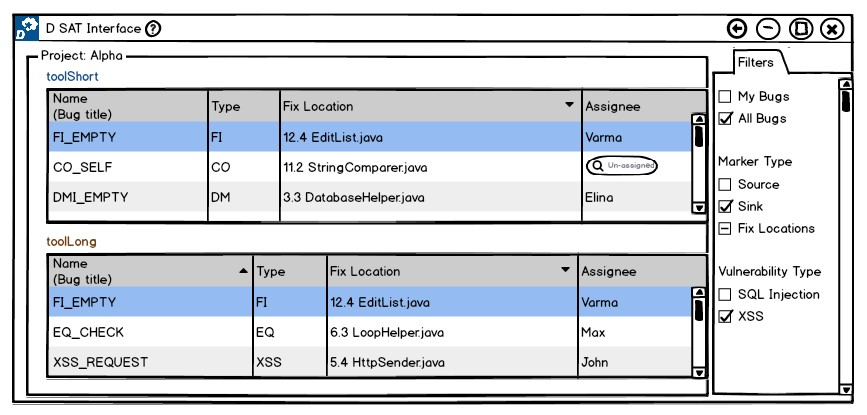
\includegraphics[width=\linewidth]{figures/d_seperate}
	\caption{An interface prototype with tools displaying results separately.}
	\label{fig:toolSeperate}
\end{figure}
\newpage

\textbf{Prototype 2}: \\ \\

The prototype for solution idea i.e., combining the results is shown in following figure \ref{fig:toolCombine}. \\ \\

\begin{figure}[hbt!]
	\centering
	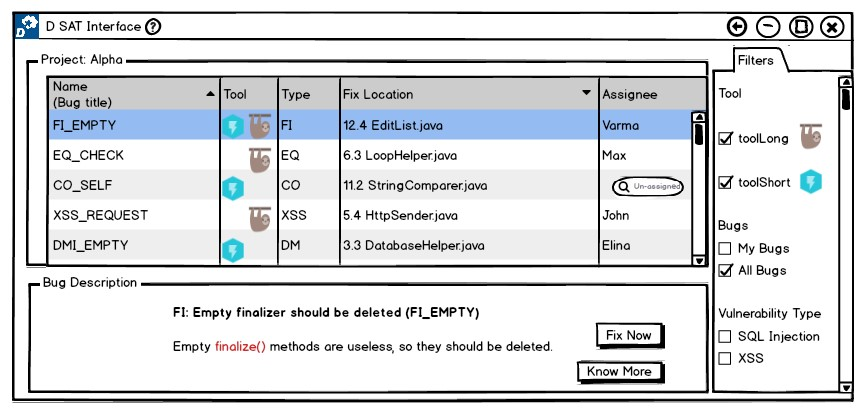
\includegraphics[width=\linewidth]{figures/d_combine}
	\caption{An interface prototype with tools displaying results combined.}
	\label{fig:toolCombine}
\end{figure}

Next, once the prototypes are designed, they are evaluated as mentioned in chapter \ref{ch:evaluationplan}. After evaluation, requirements are gathered based on user feedback and also new findings from the literature, if any. New designs are prototyped as mentioned above and repeats as per User Experience Design cycle. \\ \\

\section{Research Question 2: \\ What Feedback Works to Know that the Bug Fixing is \\ On-going?} 

\textbf{Solution ideas}: \\ \\
1. Once the user attempts to fix a bug and submit for analysis, then the bug is shown as pending in status. \\
2. If the bug is fixed then it is shown as 'fixed' in status, or else, 'try again'. \\ \\

With the above mentioned possible solution ideas, the prototypes are designed. The first prototype \ref{fig:d_pending} illustrates a bug being displayed as 'pending' in the status column of bug listing. This happens when a user selects a bug and attempts to fix it then submit for analysis tools. Perhaps the shorter tool i.e., the tool capable of analysing in less computation time would report back whether the bug is fixed or not. Thereby, the Prototype 2 \ref{fig:d_tryagain} illustrates the bug is not fixed and shown as 'try again' in status column as the user attempted to fix earlier. \\ \\

Also, in Prototype 1 it is observed that 'Fix Now' button in 'Bug Description' window is disabled which also depicts the bug is being analysed in the background. \\  \\

\textbf{Prototype 1}

\begin{figure}[hbt!]
	\centering
	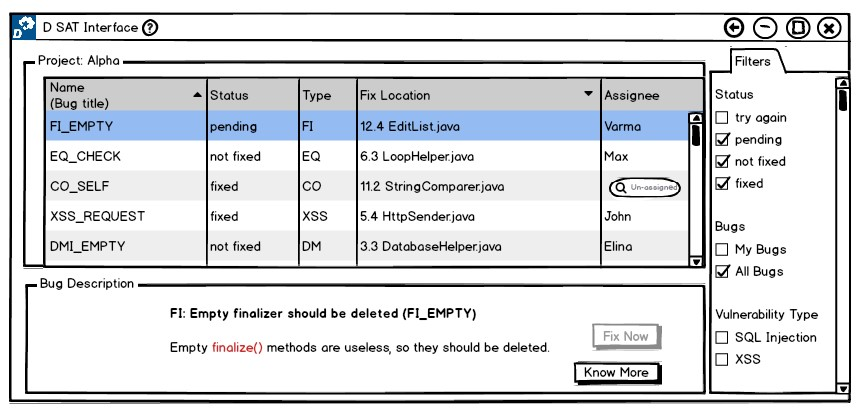
\includegraphics[width=\linewidth]{figures/d_pending}
	\caption{An interface prototype showing pending status.}
	\label{fig:d_pending}
\end{figure}

\clearpage

\textbf{Prototype 2}

\begin{figure}[hbt!]
	\centering
	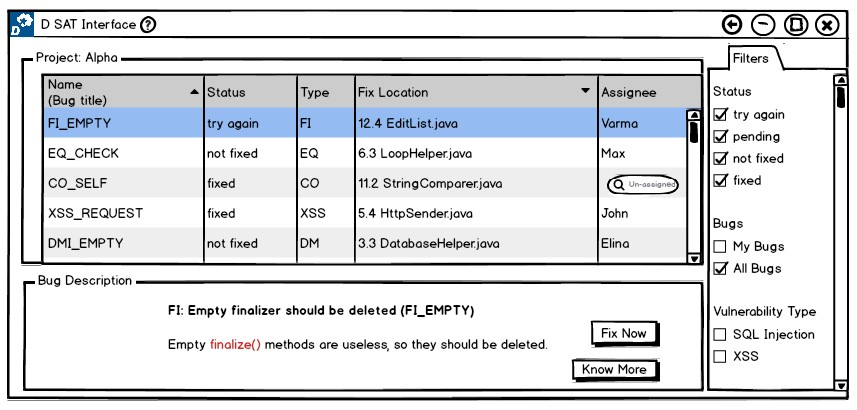
\includegraphics[width=\linewidth]{figures/d_tryagain}
	\caption{An interface prototype showing 'try again' status.}
	\label{fig:d_tryagain}
\end{figure}

Next, once the prototypes are designed, they are evaluated as mentioned in chapter \ref{ch:evaluationplan}. After evaluation, requirements are gathered based on user feedback and also new findings from the literature, if any. New designs are prototyped as mentioned above and repeats as per User Experience Design cycle. \\ \\

\section{Research Question 3:  \\ How to Carry Traceability of Bug Fixing?} 

\textbf{Solution ideas}: \\ \\
1. a time stamp for each bug fixing attempt with changes button \\
2. a Revert button \\ \\

With the above mentioned possible ideas, the prototypes are designed. The first prototype i.e., Prototype 1 \ref{fig:d_changes} illustrates there is a time stamp for each bug fixing attempt which might help in the context of traceability as to know when someone trying to mitigate a bug. Also, a button 'Changes' could perhaps show the code difference to the previous state of the codebase. The other prototype i.e., Prototype 2 \ref{fig:d_revert} illustrates in a situation where the user wants to revert back to the previous situation of the codebase. This could perhaps help in a situation when new bugs are introduced with an attempt to fix a certain bug. \\ \\

Next, once the prototypes are designed, they are evaluated as mentioned in chapter \ref{ch:evaluationplan}. After evaluation, requirements are gathered based on user feedback and also new findings from the literature, if any. New designs are prototyped as mentioned above and repeats as per User Experience Design cycle. \\ \\

\textbf{Prototype 1}
\begin{figure}[hbt!]
	\centering
	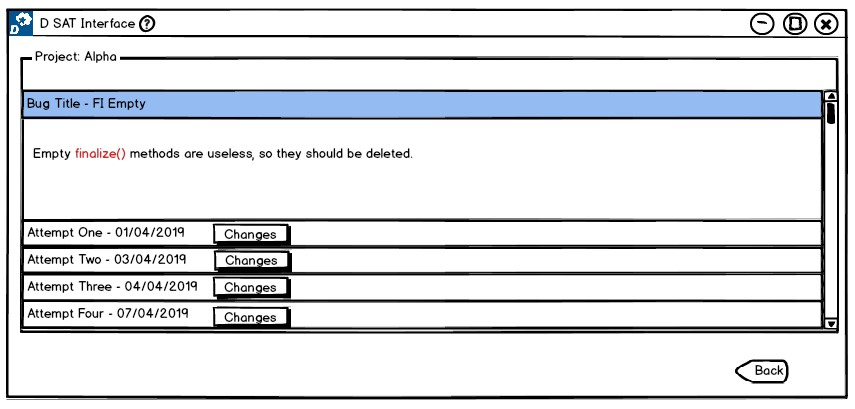
\includegraphics[width=\linewidth]{figures/d_changes}
	\caption{An interface prototype showing time stamp and changes button.}
	\label{fig:d_changes}
\end{figure}

\textbf{Prototype 2}
\begin{figure}[hbt!]
	\centering
	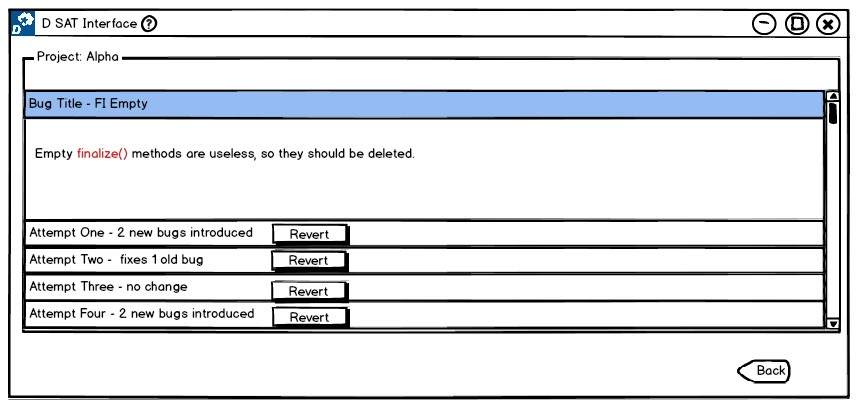
\includegraphics[width=\linewidth]{figures/d_revert}
	\caption{An interface prototype showing revert button.}
	\label{fig:d_revert}
\end{figure}

\let\cleardoublepage\clearpage